\documentclass[10pt,conference]{IEEEtran}

\usepackage{booktabs} 
\usepackage{graphicx}
\usepackage{subcaption}
\usepackage{caption}
\usepackage{url}
\usepackage{cite}
\usepackage{parcolumns}
\usepackage{listings}
\usepackage{minted}
\usepackage{xcolor}
\usepackage{algorithm2e}

\definecolor{light-gray}{gray}{0.95}

\title{
	Evaluation of Sarsa(\(\lambda\)) Learning Agent 
	}

\author{
	\IEEEauthorblockN{Padraic Cashin \IEEEauthorrefmark{1}, 
		David Lahtinen \IEEEauthorrefmark{2}, 
		Ruihao Zhou \IEEEauthorrefmark{3},
	}
	\IEEEauthorblockA{
		\IEEEauthorrefmark{1} ASU ID: 1214153888 \\
		\IEEEauthorrefmark{2} ASU ID: 1207725034 \\
		\IEEEauthorrefmark{3} ASU ID: 1213439264 \\
	}
}

% \date{}

\begin{document}
\maketitle

\section{Introduction}
\label{sec:intro}

\section{Background}
\label{sec:background}
	
	The Sarsa algorithm belongs to an On-Policy algorithm for TD-Learning. The 
	speciality of this algorithm compared to Q-Learning is that in the next 
	state, maximum reward doesn’t play an role for updating the Q-values. 
	Instead, it uses the next action and the same policy that determined the 
	original action to get new reward. The name Sarsa actually comes from the 
	four first letter of Q(s, a, r, s', a'). s and a represent original state 
	and action, r is the reward observed in the following state, s', a' are 
	the new state-action pair. As you can see in the following pictures, two 
	action selection steps needed for determining the next state-action pair 
	along with the first. The parameters a and r won’t change as they do in 
	Q-Learning. The nature of the policy's dependence on \(\mathcal{Q}\) determine 
	the convergence of the properties of Sarsa algorithm. For example, one 
	could use \(\epsilon\)-soft or \(\epsilon\)-greedy policies. \cite{sutton18} 
	
	\begin{algorithm}
		\DontPrintSemicolon
		Initialize \(Q(s,a) = 0\) for all \(s \in \mathcal{S}, a \in \mathcal{A}(s)\)\;
		\For{each episode} {
			\(E(s, a) = 0\) for all \(s \in \mathcal{S}, a \in \mathcal{A}(s)\)\;
			Initialize \(S,A\)\;
			\For{step in an episode}{
				Take action \(A\) and observe \(S',R\)\;
				Choose \(A'\) based on \(S'\) and current policy\;
				\(\delta \leftarrow R + \gamma Q(S',A') - Q(S,A)\)\;
				\(E(S,A) \leftarrow (1-\alpha) E(S,A) + 1\)\;
				\For{all \(s \in \mathcal{S}, a \in \mathcal{A}(s)\)} {
					\(Q(s,a) \leftarrow Q(s,a) + \alpha \delta E(s,a)\) \;
					\(E(s,a) \leftarrow \gamma \lambda E(s,a)\) \;
				}
				\(S \leftarrow S'\)\;
				\(A \leftarrow A'\)\;
			}
			Until \(S\) is terminal\;
		}
		\caption{Sarsa\((\lambda)\) Algorithm with Dutch Tracing}
		\label{sarsa}
	\end{algorithm}

\section{Sarsa(\(\lambda\) Implementation}
\label{sec:implementation}

	We chose to start with the codebase provided by UC Berkeley’s Pacman-themed AI 
	tutorial. As the SARSA-lambda algorithm requires an eligibility trace we 
	implemented this as a python dict with default value of 0, same as our Q table. 
	Unlike the Q-table, the eligibility trace must be cleared between episodes, 
	so we implemented a check for final step in the function which updated our 
	Q table to clear the eligibility trace.
    To test and demo the sarsa-lambda agent, we used a test that was built-in, 
	and used by UC berkeley which consisted of a small, gridworld maze for our 
	agent to run around in. What we found was that while the Default q agent 
	first had to random walk to the goal, then to the square in front of the 
	goal, and so on for each episode, the SARSA-lambda agent converged very 
	quickly. After a single random walk to the goal, the Q table updated almost 
	immediately to the optimal policy for the default starting position. While 
	we probably could have improved the results by implementing an 
	\(\epsilon\)-greedy function, our results for the basic set learning rate 
	worked very well.

	\begin{figure}[t]
		\begin{minted}
		[
			frame=lines,
			framesep=2mm,
			baselinestretch=1.2,
			fontsize=\tiny,
			bgcolor=light-gray,
		]{python}
def update(self, state, action, nextState, reward):
    nextAction = self.getAction(nextState)

    delta = reward + (self.discount * 
        self.values[(nextState, nextAction)]) - 
        self.values[(state, action)]
    
    self.eligibility[(state, action)] = (1 - self.alpha) * 
        self.eligibility[(state, action)] + 1

    for k, v in self.values.iteritems():
        trace = self.eligibility[k]
        self.values[k] = v + (self.alpha * delta * trace)
        self.eligibility[k] = trace * self.discount * self.y

    if not self.getLegalActions(nextState):
        self.eligibility = util.Counter()
		\end{minted}
		\caption{Implementation of \texttt{update} for Sarsa\((\lambda)\) agent.  Since \texttt{update} is called
		by the agent each time an aciton is selected, the function implements the inner loop
		of the algorithm detailed in Algorithm \ref{sarsa}.}
		\label{fig:sarsa-agent}
	\end{figure}

\section{Results}
\label{sec:results}


	\begin{figure*}[h]
		\centering
		\begin{subfigure}[b]{0.40\textwidth}
			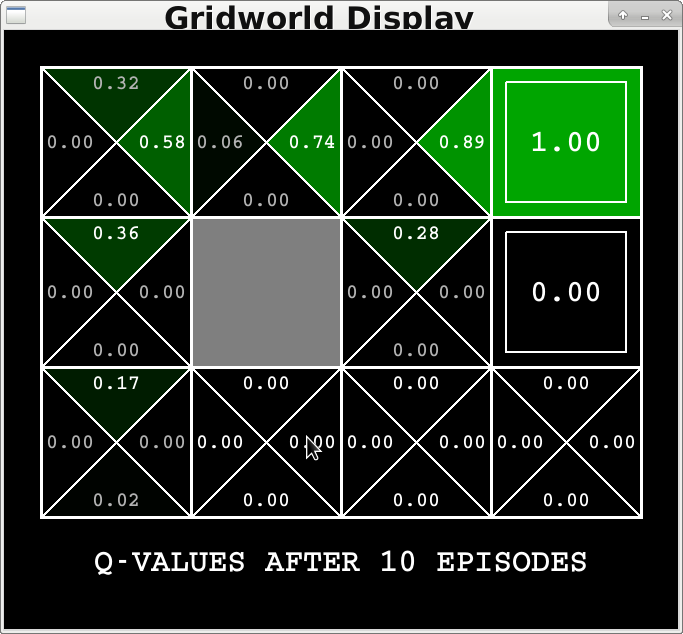
\includegraphics[width=\textwidth]{./images/qlearning_gridworld_10}
			\caption{\(Q\)-learning agent \(Q\) values}
		\end{subfigure}
		\begin{subfigure}[b]{0.40\textwidth}
			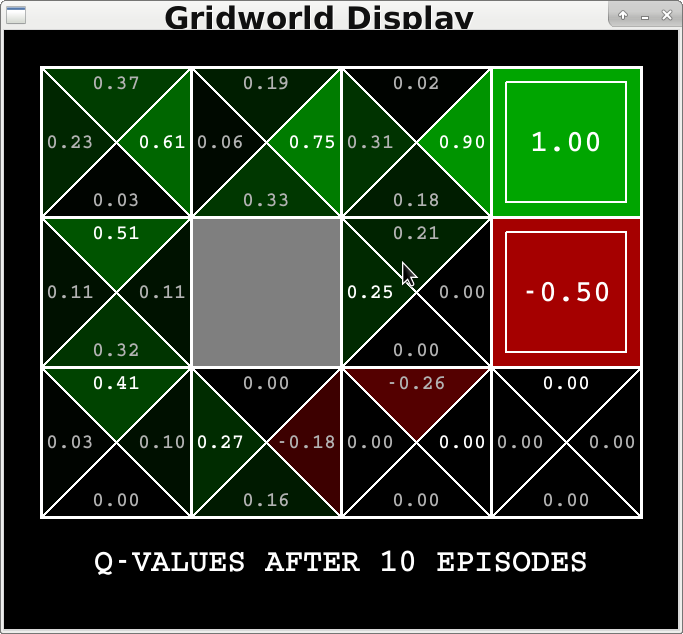
\includegraphics[width=\textwidth]{./images/sarsa_gridworld_10}
			\caption{Sarsa\((\lambda)\) agent \(Q\) values}
		\end{subfigure}
		\caption{\(Q\) values of the \(Q\)-learning and Sarsa\((\lambda)\) agents 
		after 10 episodes of traing.  The Sarsa\((\lambda)\) agent is able
		to evaluate more of the state space than the \(Q\)-learning agent.
		Each agent was run for 10 episodes on the BookGrid world with a noise
		rate of 0.2, and epsilon of 0.5.}
		\label{qvalues}
	\end{figure*}

	\begin{figure*}[h]
		\centering
		\begin{subfigure}[b]{0.40\textwidth}
			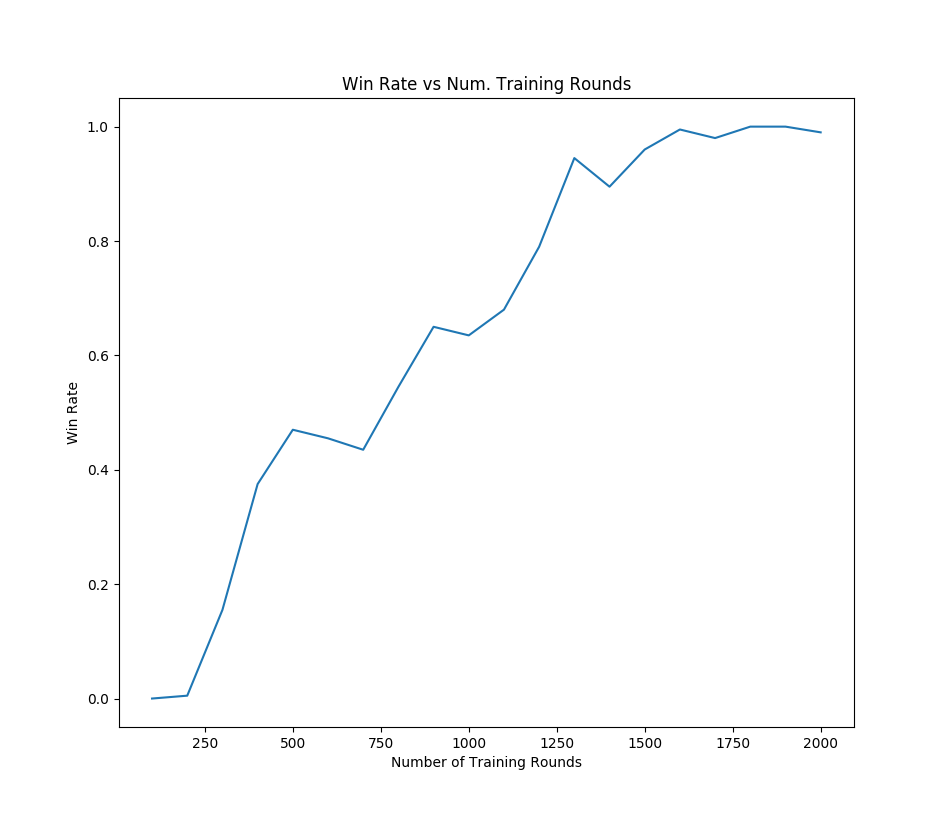
\includegraphics[width=\textwidth]{./images/qlearning_winrate}
			\caption{\(Q\)-Learning Agent}
		\end{subfigure}

		\begin{subfigure}[b]{0.40\textwidth}
			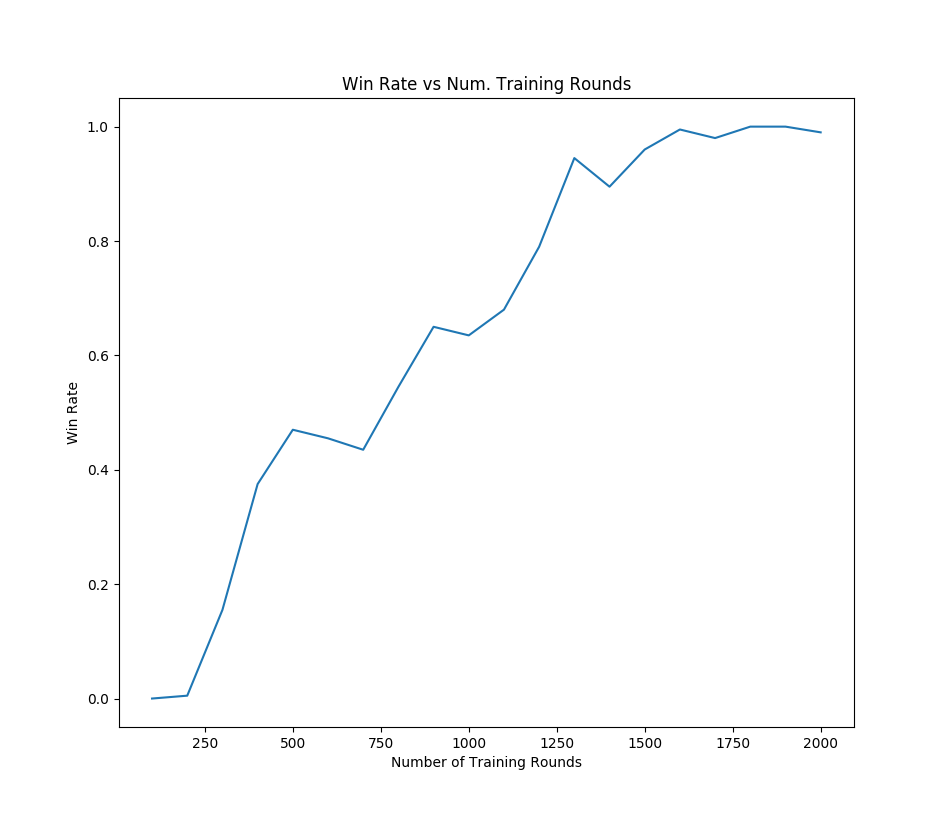
\includegraphics[width=\textwidth]{./images/qlearning_winrate}
			\caption{Sarsa\((\lambda)\) Agent}
		\end{subfigure}
		\caption{Win rate vs training episodes for \(Q\)-learning and
		Sarsa\((\lambda)\) agents.  Each agent was trained using 
		pacman smallGrid environment.  Win rate was taken from 
		20 post training episodes.}
		\label{winrate}
	\end{figure*}

\section{Conclusion}
\label{sec:conclusion}

\bibliographystyle{abbrv}
\bibliography{ref}
\end{document}












